\documentclass{article}

\usepackage{nips15submit_e,times}
\nipsfinalcopy % Uncomment for camera-ready version

% General
\usepackage[numbers]{natbib}
\usepackage{setspace}
\usepackage{geometry}
\usepackage[section]{placeins}
\usepackage[hidelinks]{hyperref}
\usepackage{graphicx}
\usepackage{color}
\usepackage{titlesec}
\usepackage[page]{appendix}
\usepackage{enumerate}

% Tables/Figures
\usepackage{lscape}
\usepackage{booktabs}
\usepackage{rotating}
\usepackage{multirow}
\usepackage{longtable}
\usepackage{caption}
\usepackage{subcaption}
\usepackage{float}

% Math
\usepackage{amsmath}
\usepackage{amssymb}
\usepackage{amsthm}
\usepackage{mathtools}
\usepackage{dsfont}

%%%%%%%%%%%%%%%%%%%%%%%%%%%%%%%%%%%%%%%%%%%%%%%%%%%%%%%%%%%%%%%%%%%%%%%%%%%%%%
% User-defined LaTeX commands
\DeclareMathOperator{\Var}{Var}
\DeclareMathOperator{\Cov}{Cov}
\DeclareMathOperator{\Corr}{Corr}
\DeclareMathOperator*{\argmax}{arg\,max}
\DeclareMathOperator*{\argmin}{arg\,min}
\DeclarePairedDelimiter{\abs}{\lvert}{\rvert}
\DeclarePairedDelimiter{\norm}{\lVert}{\rVert}
\newcommand*{\expp}[1]{\exp\left(#1\right)}
\newcommand*{\foralls}{\ \forall \ }
\newcommand*{\st}{\text{ s.t. }}
\newcommand*{\E}{\mathbb E}
\newcommand*{\R}{\mathbb R}
\newcommand*{\I}{\mathds{1}}
\newcommand*{\Prob}{\mathbb P}
\newcommand*{\convas}[1]{\xrightarrow{#1}}
\newcommand*{\conv}{\convas{}}
\newcommand*{\cond}{\;\ifnum\currentgrouptype=16 \middle\fi|\;}
\newcommand*{\defeq}{%
  \mathrel{\overset{\makebox[0pt]{\mbox{\normalfont\tiny\sffamily def}}}{=}}}
\newcommand*{\notorth}{\ensuremath{\perp\!\!\!\!\!\!\diagup\!\!\!\!\!\!\perp}}
\newcommand*{\orth}{\ensuremath{\perp\!\!\!\perp}}
\newcommand*{\evalat}{\,\big\rvert}
\newcommand*{\dif}{\,\mathrm{d}}
\newcommand*{\difto}[1]{\,\mathrm{d^#1}}
\newcommand*{\difbot}[1]{\frac{\mathrm{d}}{\mathrm{d}#1}}
\newcommand*{\partialbot}[1]{\frac{\partial}{\partial#1}}
\newcommand*{\m}[1]{\textbf{#1}}
\newcommand*{\bmath}[1]{\boldsymbol{#1}}

\newcommand*{\yestag}{\addtocounter{equation}{1}\tag{\theequation}}
\newcommand*{\notaligned}[1]{\noalign{$\displaystyle #1$}}
\newcommand*{\ttilde}{{\raise.17ex\hbox{$\scriptstyle\sim$}}}
\newcommand*{\mt}[1]{\text{\normalfont #1}}

\makeatletter
\newsavebox{\mybox}\newsavebox{\mysim}
\newcommand*{\distas}[1]{%
  \savebox{\mybox}{\hbox{\kern3pt$\scriptstyle#1$\kern3pt}}%
  \savebox{\mysim}{\hbox{$\sim$}}%
  \mathbin{\overset{#1}{\kern\z@\resizebox{\wd\mybox}{\ht\mysim}{$\sim$}}}%
}
\makeatother
\newcommand*{\dist}{\sim}
\newcommand*{\distiid}{\distas{\text{i.i.d}}}

\makeatletter
\def\moverlay{\mathpalette\mov@rlay}
\def\mov@rlay#1#2{\leavevmode\vtop{%
   \baselineskip\z@skip \lineskiplimit-\maxdimen
   \ialign{\hfil$\m@th#1##$\hfil\cr#2\crcr}}}
\newcommand*{\charfusion}[3][\mathord]{
  #1{\ifx#1\mathop\vphantom{#2}\fi\mathpalette\mov@rlay{#2\cr#3}}
  \ifx#1\mathop\expandafter\displaylimits\fi}
\makeatother
\newcommand*{\cupdot}{\charfusion[\mathbin]{\cup}{\cdot}}
\newcommand*{\bigcupdot}{\charfusion[\mathop]{\bigcup}{\cdot}}

\newtheorem{theorem}{Theorem}[section]
\newtheorem{corollary}{Corollary}[section]
\newtheorem{proposition}{Proposition}[section]
\newtheorem{lemma}{Lemma}

\theoremstyle{definition}
\newtheorem{definition}{Definition}[section]
\newtheorem{example}{Example}[section]
\newtheorem*{properties}{Properties}

\newtheoremstyle{algodesc}{}{}{}{}{\bfseries}{.}{ }{}%
\theoremstyle{algodesc}
\newtheorem{algodesc}{Algorithm}
%%%%%%%%%%%%%%%%%%%%%%%%%%%%%%%%%%%%%%%%%%%%%%%%%%%%%%%%%%%%%%%%%%%%%%%%%%%%%%

\begin{document}

\title{Annealing for Mixture Models\thanks{Stats 608A final project.}}
\author{
  Joseph Dickens \\
  University of Michigan \\
  \texttt{josephdi@umich.edu} \\
\And
  Roger Fan \\
  University of Michigan\\
  \texttt{rogerfan@umich.edu} \\
}

\maketitle


\section{Introduction} \label{sec:intro}


Mixture models are a common and powerful method for clustering and distribution estimation. Data is modeled as a ``mixture'' of multiple simple distributions, most often Gaussian, where the goal is to estimate the parameters of each distribution in the mixture. Clustering problems are unsupervised learning problems, meaning that we receive observations without knowing to which cluster they belong. Generally, mixture membership is modeled as a latent variable and parameters are estimated conditional on the latent class variable. Because the set of possible values of this latent variable can be extremely large (for instance, for $n$ data points from a two-component mixture there are $2^n$ possible latent variable realizations), direct maximization of the likelihood is generally difficult.

The most common method used to estimate parameters in this setting is the Expectation-Maximization (EM) algorithm \cite{dempsterlairdrubin77}. The EM algorithm is an iterative optimization method used to optimize a lower bound on the likelihood. There are, however, several issues with using the EM algorithm even in this fairly simple case. Mixture models often have multiple local optima. Since EM is a hill-climbing algorithm, it may converge to a local optimum rather than a global optima \cite{wu83}. This makes EM sensitive to the chosen starting point, and various ad-hoc methods (such as multiple start or random restart) are used in practice to attempt to mitigate this issue. It can also be slow to converge for a variety of reasons, including when the mixing coefficients are imbalanced or when there is significant overlap in the component distributions.

In this paper, we explore other methods that attempt to mitigate EM's issues by borrowing techniques from other optimization paradigms. Simulated annealing \cite{kirkpatrickgelattvecchi83} is of particular interest to the authors of this paper. There have been several attempts to apply annealing-inspired algorithms to mixture model estimation. Most of these methods tend to mimic EM, but replace the traditional ``E-step'' with a computationally attractive alternative. Such methods seek to explore the state space without directly hill-climbing, and possibly in a non-deterministic matter. Exploring the entire state space hopefully allows the algorithm to avoid local maxima and converge to a global maxima. The most notable algorithm is Deterministic Annealing EM (DAEM), proposed by Ueda and Nakano in 1998 \cite{uedanakano98}. As the name suggests, this algorithm replaces the stochastic nature of simulated annealing with a deterministic variant to hopefully avoid the local optima problem. Additionally, we propose a stochastic version of EM (SEM) and show that it is competitive with existing methods.


\section{Settings Where EM struggles}

Before we discuss the algorithms for estimating mixture models in section \ref{sec:algos}, we briefly describe settings where EM struggles. \cite{uedanakano98} show that when clusters have a lot of overlap, convergence of EM tends to be much slower than when clusters are well separated in the data space. Unfortunately, interesting problems are generally those with a lot of overlap, since unsupervised learning problems are much more difficult in these settings. Additionally, \cite{uedanakano98} showed that when mixing probabilities are unbalanced, meaning the data come predominantly from one class, EM can be slow to converge as well. In figure we see two comparisons that support \cite{uedanakano98} findings.


\begin{figure}[ht]
   \centering
   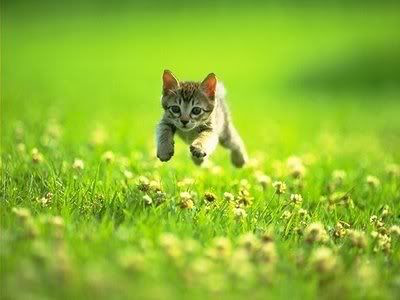
\includegraphics[width=.5\textwidth]{kitten.png}
   \label{em}
   \caption{EM is slower under these settings...}
\end{figure}

\section{Previous Algorithms} \label{sec:algos}


\subsection{Expectation-Maximization}

In their paper first proposing the general EM Algorithm \cite{dempsterlairdrubin77}, Dempster et. al. demonstrate its applicability to mixture model estimation. Due to EM's easy implementation and nice theoretical properties, EM is the standard method of estimating parametric finite mixture models. We quickly review the EM algorithm for estimating finite Gaussian mixture models as it forms the basis of the other methods.

Assume that data vectors $X_1, \dots, X_n$ are i.i.d. draws from the $J$-component mixture distribution
\begin{equation*}
P(X) = \sum_{j=1}^J \pi_j P_j(X \cond \theta_j)
\end{equation*}
Where $\pi_j$ are the mixing components, $P_j$ are the individual probability distributions, each indexed by a parameter vector $\theta_j$. Note that we can reparameterize this model by introducing a latent variable $Z$ that indicates group membership. Then our data generating model becomes:\footnote{Note that $\mt{Mult}(\cdot)$ here refers to the Multinomial distribution with $n=1$ trials, otherwise known as the Categorical distribution.}
\begin{align*}
Z &\dist \mt{Mult}(\pi_1, \dots, \pi_J) \\
X \cond Z &\dist P_Z
\end{align*}
For simplicity, in this paper we will assume that the base distributions are multivariate Gaussian, so the parameters are $\theta_j = (\mu_j, \Sigma_j)$. Gaussian mixture models are by far the most commonly used in practice, but the algorithms and methods in this paper should all generalize to any base distributions.

To estimate this model, we can use the EM algorithm as follows:
\begin{enumerate}
\item Initialize parameters for each distribution $\mu_j^{(0)}$, $\Sigma_j^{(0)}$, and mixing components $\pi_j^{(0)}$.
\item Iterate the following steps until convergence or a computing budget is met:
  \begin{enumerate}
  \item E-step: Estimate the membership probabilities $p_{ij}^{(k+1)}$ for each observation $i$ using the current parameter estimates $\mu_j^{(k)}$, $\Sigma_j^{(k)}$ and mixing components $\pi_j^{(k)}$.
    \begin{equation} \label{eq:em_estep}
    p_{ij}^{(k+1)} = P(Z_i = j \cond X_i, \mu^{(k)}, \Sigma^{(k)}, \pi^{(k)})
      = \frac{\pi_j^{(k)} P_j(X_i \cond \mu_j^{(k)}, \Sigma_j^{(k)})}{\sum_{j'=1}^J \pi_{j'}^{(k)} P_{j'}(X_i \cond \mu_{j'}^{(k)}, \Sigma_{j'}^{(k)})}
    \end{equation}
  \item M-step: Estimate the parameters and mixing components using maximum likelihood estimation conditional on the current membership probabilities.
    \begin{equation} \label{eq:em_mstep}
    \begin{gathered}
    \pi_j^{(k+1)} = \frac{1}{n} \sum_{i=1}^n p_{ij}^{(k+1)} \qquad
    \mu_j^{(k+1)} = \frac{\sum_{i=1}^n p_{ij}^{(k+1)} X_i}{\sum_{i=1}^n p_{ij}^{(k+1)}} \\
    \Sigma_j^{(k+1)} = \frac{\sum_{i=1}^n p_{ij}^{(k+1)} (X_i - \mu_j^{(k+1)}) (X_i - \mu_j^{(k+1)})'}{\sum_{i=1}^n p_{ij}^{(k+1)}}
    \end{gathered}
    \end{equation}
  \end{enumerate}
\end{enumerate}


\subsection{Deterministic Annealing}

Ueda and Nakano proposed a modification of the EM algorithm that they call Deterministic Annealing Expectation Maximization (DAEM) \cite{uedanakano98}. This algorithm is inspired by both simulated annealing and the EM algorithm, and introduces an inverse temperature parameter $\beta$ that determines how ``smoothed'' the clusters are. The DAEM algorithm is the same as EM, except replacing Equation~\ref{eq:em_estep} (the E-step) with
  \begin{equation} \label{eq:da_estep}
  p_{ij}^{(k+1)}
    = \frac{\left( \pi_j^{(k)} P_j(X_i \cond \mu_j^{(k)}, \Sigma_j^{(k)}) \right)^{\beta_k}}{\sum_{j'=1}^J \left( \pi_{j'}^{(k)} P_{j'}(X_i \cond \mu_{j'}^{(k)}, \Sigma_{j'}^{(k)}) \right)^{\beta_k}}
  \end{equation}

Note that when $\beta = 0$ the posterior membership probabilities become uniform, and when $\beta = 1$, we recover the standard EM algorithm. Generally we choose $\beta_0$ to be small, which does some smoothing between clusters, and allow $\beta_k \to 1$ as our iterations increase.


\section{Simulated Annealing}

Simulated annealing is a stochastic optimization algorithm designed to find global optima in optimization problems with large state spaces \cite{kirkpatrickgelattvecchi83}. Consider the maximization problem
\begin{equation*}
x^* = \argmax_{x \in \Omega} f(x)
\end{equation*}
The general simulated annealing algorithm proceeds as follows:
\begin{enumerate}
\item Initialize at some point $x^{(0)}$ and initial temperature $T_0$.
\item Repeat until a computing budget is met:
  \begin{enumerate}
  \item Consider some stochastically chosen candidate point $x = g(x^{(k)})$.
  \item If $f(x) > f(x^{(k)})$, accept the candidate move and set $x^{(k+1)} = x$.
  \item Otherwise, accept the candidate move with probability $e^{(f(x) - f(x^{(k)})/T_k}$.
  \item If the candidate move is not accepted, then stay at the current point $x^{(k+1)} = x^{(k)}$.
  \item Cool the temperature $T_{k+1} = \alpha T_k$ for some $0 \ll \alpha < 1$.
  \end{enumerate}
\end{enumerate}

Note that the current temperature $T_k$ determines how willing the algorithm is to accept moves that lower the objective function. For high temperatures, the algorithm accepts almost any move and uses this to explore the state space. As the temperature cools, the algorithm tends towards objective-improving moves and hopefully converges to the global optima.

In order to apply this algorithm to mixture models, we consider possible values of the latent mixture membership variable $Z$ as the state space to optimize over. Given a realization of $Z$, we can write the log-likelihood function as
\begin{equation*}
\log P(X) = \sum_{i=1}^n \sum_{j=1}^J \I(Z_i = j) \log P_j(X_i \cond \theta_j)
\end{equation*}
Plugging in the MLE estimates for $\theta_j$ conditional on $Z$, we therefore can apply simulated annealing to the objective function
\begin{equation} \label{eq:sa_obj}
f(Z) = \sum_{i=1}^n \sum_{j=1}^J \I(Z_i = j) \log P_j(X_i \cond \hat{\theta}_j)
\end{equation}


In order to implement simulated annealing to estimate mixture models, we must find a method of selecting new candidate realizations of $Z$. The implementation that adheres most closely to the traditional simulated annealing algorithm stated above randomly selects one observation and switches its membership. In this practice we found that the number of switches required to to achieve convergence made the method uncompetitive with existing algorithms. Instead, we will again draw inspiration from the EM algorithm in order to develop a simulated annealing approach that updates the entire dataset at once.


\subsection{Stochastic EM}

We propose a new algorithm that we call Stochastic EM (SEM). This is an implementation of simulated annealing that randomly draws new realizations for the entire $Z$ vector at each iteration. The SEM algorithm roughly follows the same structure as the EM algorithm:
\begin{enumerate}
\item Initialize parameters for each distribution $\mu_j^{(0)}$, $\Sigma_j^{(0)}$, mixing components $\pi_j^{(0)}$, and choose an initial temperature $T_0$.
\item Iterate the following steps until a computing budget is met:
  \begin{enumerate}
  \item Estimate the membership probabilities $p_{ij}^{(k+1)}$ using the current parameter estimates $\mu_j^{(k)}$, $\Sigma_j^{(k)}$ and mixing components $\pi_j^{(k)}$. Note that this is the exact same calculation as Equation~\ref{eq:em_estep}, the E-step from the EM algorithm.
  \item Randomly draw candidate memberships $\tilde{Z}=\left[\tilde{Z}_1,\ldots,\tilde{Z}_n\right]^T$ vector, where
    \begin{equation*}
    \tilde{Z}_i \dist \mt{Mult}\left(p_{i1}^{(k+1)}, \dots, p_{iJ}^{(k+1)}\right)
    \end{equation*}
  \item Estimate candidate parameters and mixing components using maximum likelihood estimation conditional on the memberships $\tilde{Z}$. This is analagous to the M-step in EM (\ref{eq:em_mstep}).
    \begin{equation} \label{eq:sa_mstep}
    \begin{gathered}
    \tilde{\pi}_j = \frac{1}{n} \sum_{i=1}^n \I(\tilde{Z}_i = j) \qquad
    \tilde{\mu}_j = \frac{\sum_{i=1}^n \I(\tilde{Z}_i = j) X_i}{\sum_{i=1}^n \I(\tilde{Z}_i = j)} \\
    \tilde{\Sigma}_j = \frac{\sum_{i=1}^n \I(\tilde{Z}_i = j) (X_i - \tilde{\mu}_j) (X_i - \tilde{\mu}_j)'}{\sum_{i=1}^n \I(\tilde{Z}_i = j)}
    \end{gathered}
    \end{equation}
  \item Calculate the candidate objective function
    \begin{equation*}
    f(\tilde{Z}) = \sum_{i=1}^n \sum_{j=1}^J \I(\tilde{Z}_i = j) \log P_j(X_i \cond \tilde{\mu}_j, \tilde{\Sigma}_j)
    \end{equation*}
  \item Update:
    \begin{enumerate}
    \item If $f(\tilde{Z}) > f(Z^{(k)})$ then accept the candidate memberships and update
      \begin{align*}
      Z^{(k+1)} &= \tilde{Z} & \pi^{(k+1)} &= \tilde{\pi} \\
      \mu^{(k+1)} &= \tilde{\mu} & \Sigma^{(k+1)} &= \tilde{\Sigma}
      \end{align*}
    \item Otherwise, acccept the candidate memberships with probability $e^{(f(x) - f(x^{(k)})/T_k}$.
    \item If the candidate move is not accepted, then stay at the current point $Z^{(k+1)} = Z^{(k)}$.
    \end{enumerate}
  \item Cool the temperature $T_{k+1} = \alpha T_{k}$.
  \end{enumerate}
\end{enumerate}

Comparing this to the regular EM algorithm, this is effectively a discrete, stochastic version. Instead of using the membership probabilities, SEM only allows for discrete memberships and randomly chooses memberships at each iteration using the estimated probabilities. Due to this inaccuracy, we expect that the SEM will lose some convergence speed relative to standard EM, but hope that its discrete and stochastic nature will help it avoid local optima and saddle points.



\section{Results}


\subsection{Data Generation}
\subsection{Estimation}
\subsection{Additional Simulations}

\section{Conclusion}



% \vfill
% \FloatBarrier \pagebreak
% \nocite{*}
\bibliographystyle{unsrt}
\bibliography{biblio}


\end{document}
